\section{Гипероктаэдральные комбинаторные виды}
\subsection{Определение}
Рассмотрим категорию $\HSet$. В ней объекты это множества, снабженные
дополнительным действием --- инволюцией. А стрелки, это морфизмы, сохраняющие инволюцию. 
Рассмотрим категорию $\HB$ --- подкатегорию конечных множеств из
$\HSet$ с морфизмами только биекциями, и инволюциями без неподвижных точек.
Функтор $F:\HB \rightarrow \HSet$ --- гипероктаэдральный (или кубический)
это комбинаторный вид. Мы будем так же для краткости употреблять термин
\emph{h-species}. Группоид $\HB$ эквивалентен группойду, объекты которого $\Bar
n = \{-n, -n+1, \dots, -1, 1, 2, \dots, n-1, n\}$, инволюция - смена знака.
$\Bar n$ мы интрепретируем как грани куба, на которых действует
гипероктаэдральная группа $B_n$ --- группа движений n-мерного куба.
Эта же группа действует на множестве $F[\Bar n]$, которое мы
интрепретируем как множество структур на множестве граней куба. Действие
$B_n$ возникает из перестановок граней.

\begin{example}
Вид $\mathbb H$ --- структура куб. Он сопоставляет $\Bar n$ одно множество. Все
элементы $B_n$ переходят в тождественное отображение.
\end{example}
\begin{example}
$\dA$ --- неразличимая пара граней ($\mathbb H_1$). $\dB$ --- различимая пара
граней.
Оба они принимают значение $\emptyset$ на всем, кроме $\Bar 1$. Второе
соответствует действию $H_1$ на 2-х точечном множестве.
\end{example}
\begin{example}
Аналогично $\dAA$ --- структура куб размерности 2 ($\mathbb H_2$). $\dBB$ ---
куб размерности 2 с различимыми противоположными гранями.  Второе
соответствует действию $H_2$ на 4-х точечном множестве.
\end{example}
\begin{example}
Структура $\dB \times \dB$. Это не то же самое что \dBB, поскольку это <<упорядоченная пара \dB>>.
\end{example}

\subsection{Вложение species в h-species}
Обычные комбинаторные виды можно <<вложить>> в гипероктаэдральные. Иными
словами можно каждый species рассмотреть как h-species. Для этого достаточно
рассматривать структуру не на точках, а на парах (неразличимых) граней. Если
$F:\B \rightarrow \Set$, то $\tilde{F}: \HB \rightarrow \HSet$, где
$\tilde{F}[\Bar n] = F[n]$ как множество, а инволюция тождественна.
[TODO] $HB -> B$ 

\subsection{Сложение и умножение h-species}
Сложение и умножение определяются полностью аналогично species и тут проблем не
возникает. Они введены в работе \cite{BergH}.
\begin{remark}
При работе со species, мы имели мощную комбинаторную интуицию, которая
мотивировала категорные конструкции. В случае h-species мы переносим категорные
конструкции species на новый контекст и пытаемся дать комбинаторную
интерпретацию получившимся результатам.
\end{remark}


\subsection{Аналитический функтор для h-species}
Хочется построить аналог аналитического функтора для h-species. Мы считаем, что
правильная версия гипероктаэдрального аналитического функтора действует из
$\HSet$ в $\HSet$. По аналогии с обычным случаем строим $\mathcal F$ как
расширение Кана:

\begin{tikzpicture}
\label{comm:h-an}
	\node (B) {$HB$};
	\node (S1) [below of=B] {$HSet$};
	\node (S2) [right of=B, node distance=3cm] {$HSet$};
	\draw [right hook->] (B) to node [swap] {$i$} (S1);
	\draw [->] (B) to node {$F$} (S2);
	\draw [->] (S1) to node [swap] {$\mathcal F$} (S2);
\end{tikzpicture}

Аргумент $\mathcal F$ будем называть множеством цветов.

\begin{equation}
\label{eq:h-an}
	\mathcal F(A) = \sum\limits_n F[\Bar n] \times A^{\Bar n} / B_n
\end{equation}
[TODO:Здесь нужно добавить ссылку на общую конструкцию]

$A^{\Bar n}$ --- это отображения(раскраска), сохраняющие инволюцию. По
аналогии с обычным, случаем мы мыслим $\mathcal F(A)$, как множество
$F$-структур, раскрашеных в цвета из $A$.
\begin{remark}
В новой ситуации множество цветов $A$ уже является не просто множеством, а
множеством с инволюцией. Пара элементов $(-i, i)$ отображается либо
в один и тот же элемент $(a, a)$ (который инволюцией переводится в себя), либо
в пару элементов $(b, \Bar b)$, сопряженных инволюцией. Будем называть первый
случай \emph{моноцветом}, второй --- \emph{бицветом}.
\end{remark}

Таким образом на $F[\Bar n] \times A^{\Bar n}$ действует группа $B_n \times
\mathbb Z_2$, второй сомножитель соответствует инволюции на цветах. После
факторизации по $B_n$, мы получаем $HSet$, множество с инволюцией.


%\begin{definition}
%Будем называть элементы $(F[\Bar n] \times
%A^{\Bar n})$ $A$-крашенными $F$ структурами на гранях $n$-мерного куба. Таким
%образом правую часть \ref{eq:h-an} можно интерпретировать как всевозможные
%классы эквивалентности крашеных структур.
%\end{definition}

\subsection{Декатегорификация аналитического функтора} 
Можно действовать наивно: написать производящую функцию для числа раскрасок, по
аналогии с классическим случаем. Такая формула (\ref{eq:h-fr1}) рассматривалась
(в контексте теории представлений группы $S_n \wr G$) в работе
\url{http://www.combinatorics.org/ojs/index.php/eljc/article/download/v11i1r56/pdf}
(см. также приложение B во втором анлгийском издании книги Макдональда
\cite{Mac2}). При таком подходе определяются операции сложения и умножения
по Коши для цикленных индексов. Но попытки определить
гипероктаэдральных плетизм оказываются безуспешны. Выяснилось, что правильный аналог цикленного
индекса должен помнить информацию о следующем свойстве раскрашенной структуры.

Покрашенные структуры сами по себе можно рассматривать как моноцвет, либо
бицвет. Это по--прежнему определяется длинной орбиты инволюции на $A$, уже
после факторизации по $B_n$. То есть кроме действия $B_n$ есть еще внешняя
инволюция --- действие $Z_2$. Будем разделять раскрашенные структуры на
\emph{моноструктуры} и \emph{биструктуры}.

[TODO: (расписать слово считающий) Цикленный индекс, считающий только
моноструктуры будем обозначать $\mathcal Z^{(1)}$, биструктуры --- $\mathcal Z^{(2)}$. ]

\begin{remark}
Таким образом, цикленный индекс для h-species представляет собой пару $(\Zone,
\Ztwo)$.
\end{remark}
\begin{statement}
Количество орбит под действием $B_n \times \mathbb Z_2$ соответствует $\mathcal
Z^{(1)} + \mathcal Z^{(2)}$, а под действием только $B_n$ соответствует $\mathcal Z^{(1)} + 2\mathcal
Z^{(2)}$. 
\end{statement}
\begin{proof}
В первом случае каждая моноструктура и биструктура будет посчитана 1 раз.
А во втором каждая биструктура будет посчитан два раза, т.к. действие инволюции
<<склеивающей>> две части биструктуры не учтено.
\end{proof}

\subsubsection{Подсчет цикленного индекса}
В качестве H-множества цветов возьмем счетное множество моноцветов $x_1, x_2,
x_3, \dots$ объединенное с счетным множеством бицветов $y_1, y_2, y_3, \dots$.

Допустим, что мы придумали весовую функцию, отправляющую каждую раскрашенную
структуру в моном и любая орбита отправляеться в один моном. Применив Лемму
Бернсайда переходим к подсчету неподвижных точек. Циклы в каждом элементе $B_n$
бывают двух типов:
\emph{длинные} --- каждая грань входит в цикл вместе со своей противоположной
гранью и \emph{короткие} --- пара граней лежит в симметричных, различных циклах. 

Посчитаем количество неподвижных точек для $B_n$. Пусть $\lambda^1$~
--- цикленный тип коротких перестановок, $\lambda^2$ --- цикленный тип длинных
перестановок. 
\begin{statement}
Неподвижные раскрашенные структуры, это в точности
те, у которых длинный цикл покрашен в моноцвету, а пара симметричных коротких 
может быть покрашена либо в моноцвет, либо в бицвет. 
\end{statement}
Под покрашенным циклом мы подразумеваем покраску всех его элементов в этот цвет
(такая покрашенная структура будет неподвижна относительно действия этого
элемента $B_n$).

\begin{statement}
Справедлива формула:
\begin{equation}
\label{eq:h-fr1}
\begin{split}
\mathcal Z_F^{(1)} + 2\mathcal Z_F^{(2)} = 
\sum_{n}\frac{1}{2^{n}n!}\sum_{\sigma \in B_n}&\chi(\sigma)
\psi_{x, y, y}^{\lambda^1(\sigma)} \psi_{x}^{\lambda^2(\sigma)} = \\
\sum_{n, \lambda^1 + \lambda^2 \vdash n}&\chi(\sigma_{\lambda^1 \lambda^2})
\frac{\psi_{x, y, y}^{\lambda^1} \psi_{x}^{\lambda^2}}{z_{\lambda^1 \lambda^2}}
\end{split}
\end{equation}
\end{statement}
Здесь нижний индекс $\psi$ означает переменные по которым берется степенная
сумма. Например $\psi_{x, y, y}^2 =  (x_1^2 + x_2^2 + x_3^2 + \dots + y_1^2 +
y_2^2 + y_3^2 + \dots + y_1^2 + y_2^2 + y_3^2 + \dots)$. При этом коофициент
2 у $y_i^2$ отражает тот факт, что можно раскрасить $k$ пар граней в бицвет,
так чтобы раскраска была неподвижна, под действием короткого цикла, 2-мя способами.

Посчитаем количество неподвижных точек для $B_n \times Z_2$. Разобъем
сумму на две части --- $(h, \Bar 0)$ и $(h, \Bar 1)$. Для первой формула будет
аналогична \ref{eq:h-fr1}, только из-за того что порядок группы в 2 раза больше,
появится коофициент $\frac{1}{2}$. 
Во второй части по-прежнему можно красить и длинные и короткие циклы в моноцвет.
А вот с бицветом происходит любопытная вещь --- предположим мы красим в него
цикл (пару циклов, в случае короткого). Тогда реальный цикл от $(h, \Bar 1)$
будет получатся из циклов $h$ добавлением <<смены грани>> на каждом шаге. 
Значит для циклов нечетной длинны сменится свойство короткий--длинный. 
\begin{example}
Пусть $h_e = 
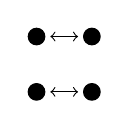
\begin{tikzpicture}
\draw [<->] (5pt, 0pt) -- (15pt, 0pt);
\draw [<->] (5pt, 20pt) -- (15pt, 20pt);
\draw[fill] (0pt,0pt) circle (3pt);
\draw[fill] (0pt, 20pt) circle (3pt);
\draw[fill] (20pt, 0pt) circle (3pt);
\draw[fill] (20pt, 20pt) circle (3pt);
\end{tikzpicture}
$.
Тогда $(h_e, \Bar 1) = 
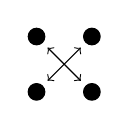
\begin{tikzpicture}
\draw [<->] (4pt, 4pt) -- (16pt, 16pt);
\draw [<->] (4pt, 16pt) -- (16pt, 4pt);
\draw[fill] (0pt,0pt) circle (3pt);
\draw[fill] (0pt, 20pt) circle (3pt);
\draw[fill] (20pt, 0pt) circle (3pt);
\draw[fill] (20pt, 20pt) circle (3pt);
\end{tikzpicture}
$
\end{example}
\begin{example}
Пусть $h_o = 
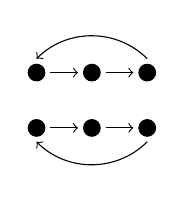
\begin{tikzpicture}
\draw [->] (5pt, 0pt) -- (15pt, 0pt);
\draw [->] (5pt, 20pt) -- (15pt, 20pt);
\draw [->] (25pt, 0pt) -- (35pt, 0pt);
\draw [->] (25pt, 20pt) -- (35pt, 20pt);
\draw [->] (40pt, -5pt) to [out=-135,in=-45] (0pt, -5pt);
\draw [->] (40pt, 25pt) to [out=135,in=45] (0pt, 25pt);
 
\draw[fill] (0pt,0pt) circle (3pt);
\draw[fill] (0pt, 20pt) circle (3pt);
\draw[fill] (20pt, 0pt) circle (3pt);
\draw[fill] (20pt, 20pt) circle (3pt);
\draw[fill] (40pt, 0pt) circle (3pt);
\draw[fill] (40pt, 20pt) circle (3pt);
\end{tikzpicture}
$.
Тогда $(h_o, \Bar 1) = 
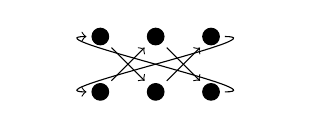
\begin{tikzpicture}
\draw [->] (4pt, 4pt) -- (16pt, 16pt);
\draw [->] (4pt, 16pt) -- (16pt, 4pt);
\draw [->] (24pt, 4pt) -- (36pt, 16pt);
\draw [->] (24pt, 16pt) -- (36pt, 4pt);
\draw [->] (45pt, 20pt) to [out=0,in=180] (-5pt, 0pt);
\draw [->] (45pt, 0pt) to [out=0,in=180] (-5pt, 20pt);
 
\draw[fill] (0pt,0pt) circle (3pt);
\draw[fill] (0pt, 20pt) circle (3pt);
\draw[fill] (20pt, 0pt) circle (3pt);
\draw[fill] (20pt, 20pt) circle (3pt);
\draw[fill] (40pt, 0pt) circle (3pt);
\draw[fill] (40pt, 20pt) circle (3pt);
\end{tikzpicture}
$
\end{example}

\begin{statement}
Справедлива формула:
\begin{equation}
\label{eq:h-fr2}
\begin{split}
\mathcal Z_F^{(1)} + \mathcal Z_F^{(2)} = 
\frac{1}{2}&
\sum_{n, \lambda^1 + \lambda^2 \vdash n}\chi(\sigma_{\lambda^1 \lambda^2})
\frac{\psi_{x, y, y}^{\lambda^1} \psi_{x}^{\lambda^2}}{z_{\lambda^1 \lambda^2}}
+ \\
\frac{1}{2}&
\sum_{n, \lambda_o^1 + \lambda_o^2 + \lambda_e^1 + \lambda_e^2 \vdash
n}\chi(\sigma_{\lambda_o^1 \lambda_o^2 \lambda_e^1 \lambda_e^2})
\frac{\psi_{x, y, y}^{\lambda_e^1 + \lambda_o^2} \psi_{x}^{\lambda_e^2 + 
\lambda_o^1}}{z_{\lambda_o^1 \lambda_o^2 \lambda_e^1 \lambda_e^2}}
\end{split}
\end{equation}
\end{statement}
Где $\lambda_o$ --- циклы нечетной длинны, $\lambda_e$ ---
циклы четной длинны.

Из формул \ref{eq:h-fr1}, \ref{eq:h-fr2} легко получить
\begin{equation}
\mathcal Z_F^{(1)} = 
\sum_{n, \lambda_o^1 + \lambda_o^2 + \lambda_e^1 + \lambda_e^2 \vdash
n}\chi(\sigma_{\lambda_o^1 \lambda_o^2 \lambda_e^1 \lambda_e^2})
\frac{\psi_{x, y, y}^{\lambda_e^1 + \lambda_o^2} \psi_{x}^{\lambda_e^2 + 
\lambda_o^1}}{z_{\lambda_o^1 \lambda_o^2 \lambda_e^1 \lambda_e^2}}
\end{equation}

\begin{equation}
\begin{split}
\mathcal Z_F^{(2)} = 
\frac{1}{2}&
\sum_{n, \lambda^1 + \lambda^2 \vdash n}\chi(\sigma_{\lambda^1 \lambda^2})
\frac{\psi_{x, y, y}^{\lambda^1} \psi_{x}^{\lambda^2}}{z_{\lambda^1 \lambda^2}}
- \\
\frac{1}{2}&
\sum_{n, \lambda_o^1 + \lambda_o^2 + \lambda_e^1 + \lambda_e^2 \vdash
n}\chi(\sigma_{\lambda_o^1 \lambda_o^2 \lambda_e^1 \lambda_e^2})
\frac{\psi_{x, y, y}^{\lambda_e^1 + \lambda_o^2} \psi_{x}^{\lambda_e^2 + 
\lambda_o^1}}{z_{\lambda_o^1 \lambda_o^2 \lambda_e^1 \lambda_e^2}}
\end{split}
\end{equation}

\subsubsection{Примеры вычисления цикленного индекса}
Посчитаем цикленные индексы для простых h-species.
Здесь мы будем писать $Z(A)$ вместо $Z_A$. Это не должно вызывать путаницу,
поскольку вместо $A$ будут использоваться схематические картинки. Их
никак не перепутать с переменными, от которых считается цикленный индекс. 
\begin{example}
$$
\Zfull(\dA) = \frac{1}{2}(\psi_{x,y,y}^1 + \psi_{x}^1) = \psi_{x,y}^1
$$
$$
\mathcal Z^{(1)}(\dA) = \frac{1}{2}(\psi_{x}^1 + \psi_{x, y, y}^1) = \psi_{x,y}^1
$$
Значит
$$
\mathcal Z^{(2)}(\dA) = 0
$$
\end{example}
\begin{example}
$$
\Zfull(\dB) = \frac{1}{2}(2\psi_{x,y,y}^1 + 0\psi_{x}^1) = \psi_{x,y,y}^1
$$
$$
\mathcal Z^{(1)}(\dB) = \frac{1}{2}(2\psi_{x}^1 + 0\psi_{x, y, y}^1) = \psi_{x}^1
$$
Значит
$$
\mathcal Z^{(2)}(\dB) = \psi_{y}^1
$$
\end{example}
\begin{example}
$$
\Zfull(\dAA) = \frac{1}{8}((\psi_{x,y,y}^1)^2 + (\psi_{x}^1)^2 + 2\psi_{x}^2 +
2(\psi_x^1\psi_{x,y,y}^1) + 2\psi_{x,y,y}^2)
$$
Здесь коофициенты --- не характеры (характер при каждом слагаемом $= 1$).
$$
\mathcal Z^{(1)}(\dAA) = \frac{1}{8}((\psi_{x}^1)^2 + (\psi_{x, y, y}^1)^2 +
2\psi_{x, y, y}^2 + 2(\psi_{x, y, y}^1\psi_{x}^1) + 2\psi_{x}^2) = \Zfull(\dAA)
$$
Последнее следовало и из общих соображений: легко видеть что $\mathcal
Z^{(2)}(\dAA) = 0$.
\end{example}
\begin{example}
$$
\Zfull(\dBB) = \frac{1}{8}(4(\psi_{x,y,y}^1)^2 + 0(\psi_{x}^1)^2 + 0\psi_{x}^2
+ 0(\psi_x^1\psi_{x,y,y}^1) + 2\times2\psi_{x,y,y}^2)
$$
$$
\mathcal Z^{(1)}(\dBB) = \frac{1}{8}(4(\psi_{x}^1)^2 + 2\times2\psi_{x,y,y}^2)
$$
Откуда
$$
\mathcal Z^{(2)}(\dBB) = \frac{1}{2}(\Zfull(\dBB) - \mathcal
Z^{(1)}(\dBB)) = \frac{1}{2}(\psi_{y,y}^1\psi_{x}^1 +
\frac{1}{2}(\psi_{y, y}^1)^2) = \psi_{y}^1\psi_{x}^1 + (\psi_{y}^1)^2 $$
\end{example}

\subsection{Сумма и произведение цикленных индексов}
\subsubsection{Сумма}
Сумма цикленных индексов соответсвует поточечной сумме аналитических
функторов и здесь нет никаких сюрпризов:
$$
\mathcal Z_{A + B}^{(1)} = \mathcal Z_A^{(1)} + \mathcal Z_B^{(1)}
$$
$$
\mathcal Z_{A + B}^{(2)} = \mathcal Z_A^{(2)} + \mathcal Z_B^{(2)}
$$
\subsubsection{Произведение}
Для произведения уже не совсем так. 
\begin{statement}
Моноструктура получается
в произведении двух моноструктур. А биструктура получается, если один из
сомножителей биструктура. Причем в случае, когда оба сомножителя ---
биструктуры, получается две различных биструктуры. 
\end{statement}
То есть
$$
\mathcal Z_{A * B}^{(1)} = \mathcal Z_A^{(1)} * \mathcal Z_B^{(1)}
$$
$$
\mathcal Z_{A * B}^{(2)} = 
\mathcal Z_A^{(1)} * \mathcal Z_B^{(2)} + 
\mathcal Z_A^{(2)} * \mathcal Z_B^{(1)} +
2 (\mathcal Z_A^{(2)} * \mathcal Z_B^{(2)})
$$
Откуда следует
$$
(\mathcal Z_{A * B}^{(1)} + 2\mathcal Z_{A * B}^{(2)}) = 
(\mathcal Z_A^{(1)} + 2\mathcal Z_A^{(2)}) * 
(\mathcal Z_B^{(1)} + 2\mathcal Z_B^{(2)})
$$

\begin{remark}
Это логично, поскольку $(\mathcal Z_F^{(1)} + 2\mathcal Z_F^{(2)})$ --- это
цикленный индекс для цветов, с <<забытой>> инволюцией.
\end{remark}

\subsubsection{Примеры цикленных индексов произведений}
Посчитаем произведение уже известных h-структур и их цикленных индексов.

\begin{example}
Структура $\dA \times \dA$.
$$
\mathcal Z^{(1)}(\dA \times \dA) = \mathcal Z^{(1)}(\dA) \times \mathcal
Z^{(1)}(\dA) = (\psi_{x, y}^1)^2
$$
\end{example}
\begin{example}
Структура $\dB \times \dB$.
$$
\Zfull(\dB \times \dB) = \Zfull(\dB) \times \Zfull(\dB) =(\psi_{x, y, y}^1)^2
$$
Легко получить эту же формулу и прямым подсчетом по формуле \ref{eq:h-fr1}, как
$\frac{1}{8}(8(\psi_{x, y, y}^1)^2)$.
$$
\mathcal Z^{(1)}(\dB \times \dB) = \mathcal Z^{(1)}(\dB) \times \mathcal
Z^{(1)}(\dB) =(\psi_{x}^1)^2
$$
\end{example}

\subsection{Цикленный индекс композиции}
\begin{problem}
Как выразить
\begin{equation*}
\begin{split}
\mathcal Z^{(i)}_{F \circ G} (&\psi_x^1, \psi_x^2, \psi_x^3, \dots, \\
						&\psi_y^1, \psi_y^2, \psi_y^3, \dots)
\end{split}
\end{equation*}
\end{problem}

[TODO: Dopisat etot razdel, поставить ссылку на основную теоерму \ref{th:z-main}]
Теперь попробуем выстроить теорию композиции цикленного индекса для h-species,
параллельно теории species. В качестве моноцветов возьмем $\{x_1, x_2, x_3,
\dots\}$, бицветов --- $\{y_1, y_2, y_3, \dots\}$. Формулы \ref{eq:h-fr1} и
\ref{eq:h-fr2} подсказывают, что на практике в качестве симметричного базиса
можно брать не $\{\psi_x^i, \psi_y^j\}$ а $\{\psi_x^i, \psi_{x,y,y}^j\}$. Или
другую линейную комбинацию, например $\{\psi_x^i, \psi_{x,y}^j\}$.


Биструктуры подставляются вместо бицветов, моноструктуры, вместо моноцветов. В
остальном рассуждение дословно повторяет случай обычных species.

\begin{theorem}
\label{th:z-main}
\begin{equation}
\begin{split}
\label{eq:h-zfg}
	\mathcal Z^{(i)}_{F \circ G} (\psi_x^1, \psi_x^2, \psi_x^3, &\dots, 
	\psi_y^1, \psi_y^2, \psi_y^3, \dots) = \\
	\mathcal Z_F^{(i)}(
		&\mathcal Z^{(1)}_G(\psi_x^1, \psi_x^2, \psi_x^3, \dots, 
					 \psi_y^1, \psi_y^2, \psi_y^3, \dots), \\
		&\mathcal Z^{(1)}_G(\psi_x^2, \psi_x^4, \psi_x^6, \dots, 
					 \psi_y^2, \psi_y^4, \psi_y^6, \dots), \\
		&\mathcal Z^{(1)}_G(\psi_x^3, \psi_x^6, \psi_x^9, \dots, 
					 \psi_y^3, \psi_y^6, \psi_y^9, \dots), \\
		&\dots, \\
		&\Ztwo_G(\psi_x^1, \psi_x^2, \psi_x^3, \dots, 
					 \psi_y^1, \psi_y^2, \psi_y^3, \dots), \\
		&\Ztwo_G(\psi_x^2, \psi_x^4, \psi_x^6, \dots, 
					 \psi_y^2, \psi_y^4, \psi_y^6, \dots), \\
		&\Ztwo_G(\psi_x^3, \psi_x^6, \psi_x^9, \dots, 
					 \psi_y^3, \psi_y^6, \psi_y^9, \dots), \\
		&\dots
	)
\end{split}	
\end{equation}
Эта формула слишком громоздкая, поэтому напишем ее на уровне членов:
\begin{equation*}
\begin{split}
\psi_x^i \circ (\mathcal Z^{(1)}_G, \mathcal Z^{(2)}_G ) = \Zone_G
(&\psi_x^i, \psi_x^{2i}, \psi_x^{3i}, \dots, \\
&\psi_y^i, \psi_y^{2i}, \psi_y^{3i}, \dots)
\end{split}
\end{equation*}

\begin{equation*}
\begin{split}
\psi_y^i \circ (\mathcal Z^{(1)}_G, \mathcal Z^{(2)}_G ) = \Ztwo_G
(&\psi_x^i, \psi_x^{2i}, \psi_x^{3i}, \dots, \\
&\psi_y^i, \psi_y^{2i}, \psi_y^{3i}, \dots)
\end{split}
\end{equation*}
\end{theorem}

\begin{remark}
Если сделать в \ref{eq:h-zfg} подстановку 
$$
\psi_{x}^1 = t, \psi_{x}^k = 0, k>1
$$
$$
\psi_y^1 = s, \psi_y^k = 0, k>1
$$
То получится формула
$$
\tilde{\mathcal Z}^{(i)}_{F \circ G} (t, s) = 
	\tilde{\mathcal Z}_F^{(i)} (
		\tilde{\mathcal Z}_G^{(1)} (t, s), 
		\tilde{\mathcal Z}_G^{(2)} (t, s))
$$
Таким образом аналог \ref{eq:comp} справедлив для
экспоненциальных производящих функций bilabeled-структур.
\end{remark}

\subsubsection{Примеры цикленного индекса композиции}
\begin{example}
Посчитаем $(\mathcal Z^{(1)}, \mathcal Z^{(2)})(\dB \circ \dA)$
$$
\mathcal Z^{(1)}(\dB \circ \dA) = \psi_{x}^1 \circ \psi_{x, y}^1 = \psi_{x, y}^1
= \mathcal Z^{(1)}(\dA)
$$ 
$$
\mathcal Z^{(2)}(\dB \circ \dA) = \psi_{y}^1 \circ 0 = 0 = \mathcal Z^{(2)}(\dA)
$$
\end{example}
\begin{example}
Да и вобще, справедливо
$$
\mathcal Z^{(i)}(\dB \circ A) = \mathcal Z^{(i)}(A)
$$ 
$$
\mathcal Z^{(i)}(A \circ \dB) = \mathcal Z^{(i)}(A)
$$
\end{example}
\begin{remark}
Это дает некоторое понимание композиции. Так видимо $A \circ \dB = \dB \circ A =
A$. То есть \dB является нейтральным элементом в монойде h-species по
композиции.
Это несколько контр-интуитивно, поскольку в обычных species нейтральным
элементом являеться одноточечное множество. А его образом при вложении species в
h-species являеться \dA.
\end{remark}
\begin{example}
Интересно посмотреть на композицию с \dA
\begin{equation}
\begin{split}
\Zfull(\dBB \circ \dA) = \frac{1}{2} (\frac{1}{2}(\psi_{x,y,y}^1 +
\psi_{x}^1))^2 + \frac{1}{2} (\frac{1}{2}(\psi_{x,y,y}^2 +
\psi_{x}^2)) = \\
\frac{1}{8}((\psi_{x}^1)^2 + (\psi_{x, y, y}^1)^2 +
2\psi_{x, y, y}^2 + 2(\psi_{x, y, y}^1\psi_{x}^1) + 2\psi_{x}^2) =
\Zfull(\dAA)
\end{split}
\end{equation}
\begin{remark}
Отcюда можно сделать предположение, что $\dBB \circ \dA = \dAA$.
То есть подстановка \dA~--- это <<стирание различий между противоположными
гранями>>.
\end{remark}
\end{example}
\begin{example}
[TODO:дописать]
Посчитаем для структуры $V$ <<вершина куба>>.
$$
\Zfull(V) = e^{\psi_{x,y,y}^{1} + \frac{\psi_{x,y,y}^{2}}{2} +
\frac{\psi_{x,y,y}^{3}}{3} + \dots} 
$$

$$
\mathcal Z^{(1)}(V) = e^{(\psi_{x}^{1} + \frac{\psi_{x}^{2}}{2} +
\frac{\psi_{x}^{3}}{3} + \dots) + (\psi_{y}^{2} + \frac{\psi_{y}^{4}}{2} +
\frac{\psi_{y}^{6}}{3} + \dots)} 
$$

Для структуры $H$ <<куб>>.
$$
\Zfull(H) = \mathcal Z^{(1)}(H) = e^{\psi_{x,y}^{1} +
\frac{\psi_{x,y}^{2}}{2!} + \frac{\psi_{x,y}^{3}}{3!} + \dots} 
$$
Тогда $\mathcal Z^{(i)}(V \circ \dA) = \mathcal Z^{(i)}(H)$, поскольку
при специализации всех $y$ в $0$, они равны.
\end{example}

\subsection{Цикленный индекс species, вложенных в h-species}
\begin{statement}
Пусть $G$ --- обычный species, вложенный в h-species. $\mathcal Z_G$ --- его
цикленный индекс.
$$(\mathcal Z^{(1)}_G, \mathcal Z^{(2)}_G)
(\psi_x^1, \psi_x^2, \psi_x^3, \dots, 
\psi_y^1, \psi_y^2, \psi_y^3, \dots)
 = (\mathcal Z_G(\psi_{x,y}^1, \psi_{x,y}^2, \psi_{x,y}^3, \dots), 0)$$
\end{statement}

\subsection{Применение цикленного индекса к решению задач о раскрасках}
\begin{problem}
Посчитать количество способов покрасить $n$-мерный куб в $k$ цветов с точностью
до изометрий. Иными словами, посчитать количество орбит при действии $B_n$ на
множестве всевозможно раскрашенных кубов. \url{http://math.stackexchange.com/questions/5697/coloring-the-faces-of-a-hypercube}.
\end{problem}
\begin{solution}
В нашей нотации это вопрос о количестве раскрасок пар граней в $k$ моноцветов и
$\frac{k(k-1)}{2}$ бицветов. Поскольку любая раскраска даст нам моноструктуру,
то производящая функция для количества раскрасок от размерности, будет равна
$\Zone_{\mathbb H}(kt, kt^2, kt^3, \dots, k^2t,
k^2t^2, k^2t^3, \dots) = exp(kt + kt^2 + kt^3 + \dots
+ \frac{k(k-1)}{2}t + \frac{k(k-1)}{2}t^2 + \frac{k(k-1)}{2}t^3 + \dots) =
exp(\frac{k(k+1)}{2}t + \frac{k(k+1)}{2}t^2 + \frac{k(k+1)}{2}t^3 + \dots) =
(exp(log(\frac{1}{1-t})))^{\frac{k(k+1)}{2}} = \frac{1}{1-t}^{\frac{k(k+1)}{2}}$
\end{solution}
